\documentclass[11pt]{article}
\usepackage[margin=1.05cm]{geometry}
\usepackage{amsmath,amssymb}
\usepackage{tikz}
\usepackage{tikz-cd}
\usetikzlibrary{arrows.meta,positioning,calc,fit,backgrounds,quotes,
  decorations.pathmorphing,shapes.geometric,shapes.misc,fadings}
\usepackage{caption}
\captionsetup{font=footnotesize,labelfont=bf}
\pagestyle{empty}

% ---- shared styles ----
\tikzset{
  obj/.style   ={draw,rounded corners=2pt,inner sep=3.5pt,font=\small,minimum height=6mm},
  core/.style  ={draw,rounded corners=2pt,inner sep=3.5pt,font=\small,fill=black!7,minimum height=6mm},
  ar/.style    ={-{Stealth[length=5pt]}},
  iso/.style   ={{Stealth[length=5pt]}-{Stealth[length=5pt]},thick},
  mono/.style  ={{Hook[right,length=4pt]}-{Stealth[length=5pt]}},
  epi/.style   ={-{Stealth[length=5pt] Stealth[length=5pt]}},
  dashar/.style={-{Stealth[length=5pt]},dashed},
  dot/.style   ={circle,fill=black,inner sep=1.3pt},
  lbl/.style   ={font=\scriptsize\itshape,inner sep=1.5pt},
  tag/.style   ={font=\scriptsize,inner sep=1pt},
}
\newcommand{\fig}[2]{\begin{minipage}[t]{#1}\centering #2\end{minipage}}

\begin{document}
\begin{center}
  {\Large\bfseries A Visual Atlas of the Semantic--Bridge Library}\\[2pt]
  {\footnotesize iso $\;\cong\;$ \quad dual $\;\dashv\;$ \quad equiv $\;\simeq\;$ \quad --- patterns, drawn}
\end{center}
\vspace{-2mm}

%==================================================================
\noindent\hrulefill\\[2pt]
\begin{minipage}[t]{0.48\textwidth}\centering
% ---- 1. The fusion cospan ----
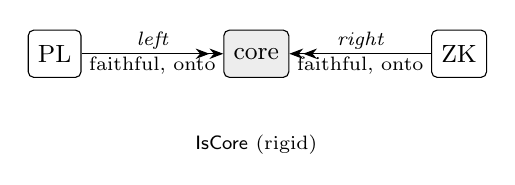
\begin{tikzpicture}[node distance=10mm]
  \node[obj] (S) {PL};
  \node[core] (C) [right=18mm of S] {core};
  \node[obj] (T) [right=18mm of C] {ZK};
  \draw[epi] (S) -- node[lbl,above]{left} node[tag,below]{faithful, onto} (C);
  \draw[epi] (T) -- node[lbl,above]{right} node[tag,below]{faithful, onto} (C);
  \node[tag] at ($(C)+(0,-1.15)$) {$\mathsf{IsCore}$ (rigid)};
\end{tikzpicture}
\captionof{figure}{\texttt{Fusion S T}: one object both worlds factor onto.}
\end{minipage}\hfill
\begin{minipage}[t]{0.48\textwidth}\centering
% ---- 2. Semantics-preserving square ----
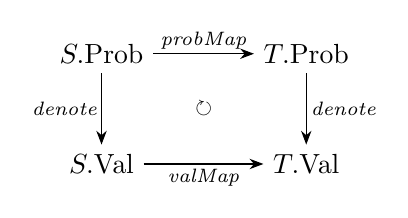
\begin{tikzpicture}
  \node (a) at (0,1.4) {$S.\mathrm{Prob}$};
  \node (b) at (2.6,1.4) {$T.\mathrm{Prob}$};
  \node (c) at (0,0) {$S.\mathrm{Val}$};
  \node (d) at (2.6,0) {$T.\mathrm{Val}$};
  \draw[ar] (a) -- node[lbl,above]{probMap} (b);
  \draw[ar] (a) -- node[lbl,left]{denote} (c);
  \draw[ar] (b) -- node[lbl,right]{denote} (d);
  \draw[ar] (c) -- node[lbl,below]{valMap} (d);
  \node[tag] at (1.3,0.7) {$\circlearrowright$};
\end{tikzpicture}
\captionof{figure}{\texttt{SchemeHom}: the square commutes (soundness, free).}
\end{minipage}

\vspace{1.5mm}
\begin{minipage}[t]{0.48\textwidth}\centering
% ---- 3. Reflection / localization triangle ----
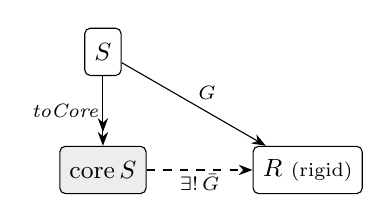
\begin{tikzpicture}
  \node[obj] (S) at (0,1.5) {$S$};
  \node[core] (C) at (0,0) {$\mathrm{core}\,S$};
  \node[obj] (R) at (2.6,0) {$R$ \scriptsize(rigid)};
  \draw[epi] (S) -- node[lbl,left]{toCore} (C);
  \draw[ar]  (S) -- node[lbl,above right]{$G$} (R);
  \draw[dashar] (C) -- node[lbl,below]{$\exists!\,\bar G$} (R);
\end{tikzpicture}
\captionof{figure}{Core = \emph{reflector}: unique factorization through \texttt{toCore}.}
\end{minipage}\hfill
\begin{minipage}[t]{0.48\textwidth}\centering
% ---- 4. Idempotence loop ----
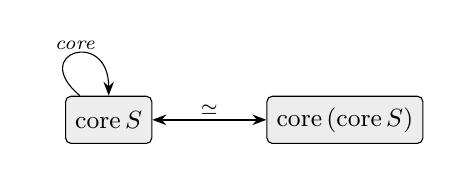
\begin{tikzpicture}
  \node[core] (C) at (0,0) {$\mathrm{core}\,S$};
  \node[core] (CC) at (3,0) {$\mathrm{core}\,(\mathrm{core}\,S)$};
  \draw[iso] (CC) -- node[lbl,above]{$\simeq$} (C);
  \draw[ar] (C) to[out=140,in=90,looseness=6] node[lbl,above]{core} (C);
\end{tikzpicture}
\captionof{figure}{Idempotent reflector: \texttt{core\,(core\,S)\,$\simeq$\,core\,S}.}
\end{minipage}

%==================================================================
\vspace{1.5mm}\noindent\hrulefill\\[2pt]
\begin{minipage}[t]{0.5\textwidth}\centering
% ---- 5. Case-split coverage / regions ----
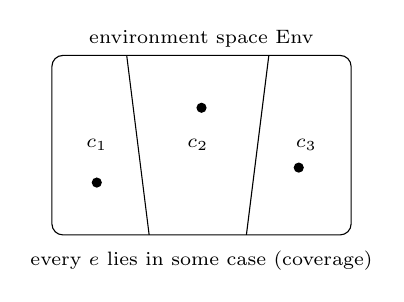
\begin{tikzpicture}[scale=0.95]
  \draw[rounded corners] (0,0) rectangle (4,2.4);
  \node[tag] at (2,2.62) {environment space $\mathrm{Env}$};
  \draw (1.3,0) -- (1.0,2.4);
  \draw (2.6,0) -- (2.9,2.4);
  \node[tag] at (0.6,1.2) {$c_1$};
  \node[tag] at (1.95,1.2) {$c_2$};
  \node[tag] at (3.4,1.2) {$c_3$};
  \node[dot] at (0.6,0.7){}; \node[dot] at (2.0,1.7){}; \node[dot] at (3.3,0.9){};
  \node[tag] at (2,-0.35) {every $e$ lies in some case (coverage)};
\end{tikzpicture}
\captionof{figure}{\texttt{CaseSplitScheme}: split $\to$ per-case decidable fragment.}
\end{minipage}\hfill
\begin{minipage}[t]{0.46\textwidth}\centering
% ---- 6. Quotient collapse ----
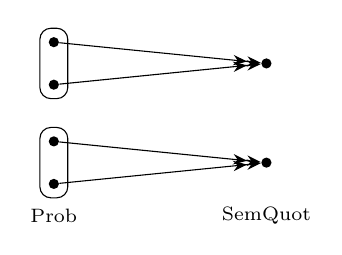
\begin{tikzpicture}[scale=0.9]
  \foreach \y/\n in {2/a,1.4/b,0.6/c,0/d}{\node[dot](L\n) at (0,\y){};}
  \node[draw,rounded corners,fit=(La)(Lb),inner sep=3pt](g1){};
  \node[draw,rounded corners,fit=(Lc)(Ld),inner sep=3pt](g2){};
  \node[dot] (R1) at (3,1.7){}; \node[dot] (R2) at (3,0.3){};
  \draw[epi] (La) -- (R1); \draw[epi] (Lb) -- (R1);
  \draw[epi] (Lc) -- (R2); \draw[epi] (Ld) -- (R2);
  \node[tag] at (0,-0.45){Prob};
  \node[tag] at (3,-0.45){SemQuot};
\end{tikzpicture}
\captionof{figure}{Collapse: $u\sim v \iff \texttt{toQuot}\,u=\texttt{toQuot}\,v$.}
\end{minipage}

\vspace{1.5mm}
\begin{minipage}[t]{0.52\textwidth}\centering
% ---- 7. Transport theorem ----
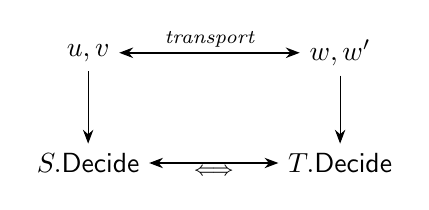
\begin{tikzpicture}
  \node (u) at (0,1.4) {$u,v$}; \node (w) at (3.2,1.4) {$w,w'$};
  \node (Su) at (0,0) {$S.\mathsf{Decide}$}; \node (Tw) at (3.2,0) {$T.\mathsf{Decide}$};
  \draw[iso] (u) -- node[lbl,above]{transport} (w);
  \draw[{Stealth[length=5pt]}-{Stealth[length=5pt]}] (Su) -- node[lbl,below]{$\Longleftrightarrow$} (Tw);
  \draw[ar] (u) -- (Su); \draw[ar] (w) -- (Tw);
\end{tikzpicture}
\captionof{figure}{Transport: a verified checker/normalizer moves world to world.}
\end{minipage}\hfill
\begin{minipage}[t]{0.44\textwidth}\centering
% ---- 8. SemEquiv groupoid ----
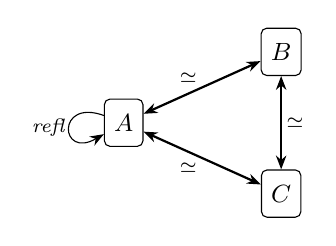
\begin{tikzpicture}
  \node[obj] (A) at (0,0) {$A$};
  \node[obj] (B) at (2,0.9) {$B$};
  \node[obj] (D) at (2,-0.9) {$C$};
  \draw[iso] (A) -- node[lbl,above left]{$\simeq$} (B);
  \draw[iso] (A) -- node[lbl,below left]{$\simeq$} (D);
  \draw[iso] (B) -- node[lbl,right]{$\simeq$} (D);
  \draw[ar] (A) to[out=160,in=210,looseness=7] node[lbl,left]{refl} (A);
\end{tikzpicture}
\captionof{figure}{\texttt{SemEquiv}: refl / symm / trans (an equivalence).}
\end{minipage}

%==================================================================
\vspace{1.5mm}\noindent\hrulefill\\[2pt]
\begin{minipage}[t]{0.55\textwidth}\centering
% ---- 9. Arithmetization iso: tree <-> trace ----
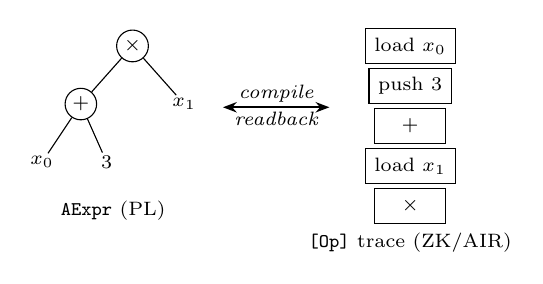
\begin{tikzpicture}[scale=0.82,every node/.style={font=\scriptsize}]
  % expression tree
  \node[circle,draw,inner sep=1.2pt] (p) at (0,2.1) {$\times$};
  \node[circle,draw,inner sep=1.2pt] (pl) at (-0.8,1.2) {$+$};
  \node[inner sep=1pt] (x) at (-1.4,0.3) {$x_0$};
  \node[inner sep=1pt] (c) at (-0.4,0.3) {$3$};
  \node[inner sep=1pt] (y) at (0.8,1.2) {$x_1$};
  \draw (p)--(pl); \draw (p)--(y); \draw (pl)--(x); \draw (pl)--(c);
  \node[tag] at (-0.3,-0.45){\texttt{AExpr} (PL)};
  % tape
  \foreach \i/\t in {0/{load $x_0$},1/{push 3},2/{+},3/{load $x_1$},4/{$\times$}}{
    \node[draw,minimum width=9mm,minimum height=4.5mm] (t\i) at (4.3,2.1-\i*0.62) {\t};}
  \node[tag] at (4.3,-0.95){\texttt{[Op]} trace (ZK/AIR)};
  \draw[iso] (1.4,1.15) -- node[lbl,above]{compile} node[lbl,below]{readback} (3.05,1.15);
\end{tikzpicture}
\captionof{figure}{Real systems: expression $\cong$ execution trace (both onto same functions).}
\end{minipage}\hfill
\begin{minipage}[t]{0.42\textwidth}\centering
% ---- 10. Duality: contravariance ----
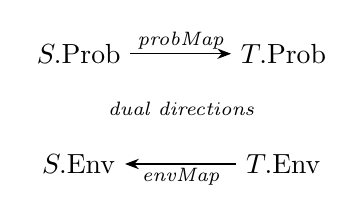
\begin{tikzpicture}
  \node (SP) at (0,1.4){$S.\mathrm{Prob}$}; \node (TP) at (2.6,1.4){$T.\mathrm{Prob}$};
  \node (SE) at (0,0){$S.\mathrm{Env}$};   \node (TE) at (2.6,0){$T.\mathrm{Env}$};
  \draw[ar] (SP) -- node[lbl,above]{probMap} (TP);
  \draw[ar] (TE) -- node[lbl,below]{envMap} (SE);
  \node[tag] at (1.3,0.7){\itshape dual directions};
\end{tikzpicture}
\captionof{figure}{Duality: objects co-, environments contra-variant.}
\end{minipage}

\vspace{1.5mm}
\begin{minipage}[t]{0.5\textwidth}\centering
% ---- 11. faithful-but-not-onto gap ----
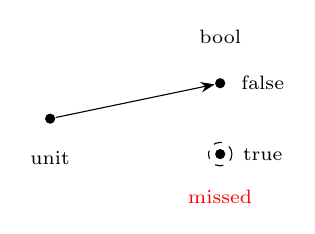
\begin{tikzpicture}[scale=0.9]
  \node[dot] (u) at (0,0.5){};
  \node[dot] (f) at (2.4,1.0){}; \node[tag] at (3.0,1.0){false};
  \node[dot] (t) at (2.4,0.0){};
  \node[draw,dashed,circle,inner sep=3pt] at (2.4,0.0){};
  \node[tag] at (3.0,0.0){true};
  \draw[ar] (u) -- (f);
  \node[tag,red] at (2.4,-0.6){missed};
  \node[tag] at (0,-0.05){unit}; \node[tag] at (2.4,1.65){bool};
\end{tikzpicture}
\captionof{figure}{Faithful $\ne$ onto: \texttt{unitToBool} misses a whole class.}
\end{minipage}\hfill
\begin{minipage}[t]{0.46\textwidth}\centering
% ---- 12. imax piecewise case ----
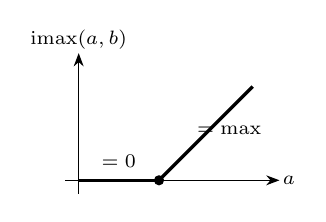
\begin{tikzpicture}[scale=0.85,>=Stealth]
  \draw[->] (-0.2,0) -- (3,0) node[right,tag]{$a$};
  \draw[->] (0,-0.2) -- (0,1.9) node[above,tag]{$\mathrm{imax}(a,b)$};
  \draw[very thick] (0,0) -- (1.2,0);
  \draw[very thick] (1.2,0) -- (2.6,1.4);
  \node[tag] at (0.6,0.28){$=0$};
  \node[tag] at (2.25,0.75){$=\max$};
  \node[dot] at (1.2,0){};
\end{tikzpicture}
\captionof{figure}{\texttt{imax}: piecewise ($0$ or $\max$) $\Rightarrow$ zero-pattern case split.}
\end{minipage}

\vspace{1mm}
\begin{center}\footnotesize
$\underbrace{\text{PL}}_{\text{normalize}}\ \xrightarrow{\ \cong\ }\ \boxed{\text{one semantic core}}\ \xleftarrow{\ \cong\ }\ \underbrace{\text{ZK}}_{\text{constraint reduce}}$
\end{center}

\end{document}
